\subsection{From Idempotent Semigroups to General Semigroups}\label{sec:noncommutative_extension}

In this section we provide a detailed explanation of the reduction in Theorem~\ref{thm:lowerbound} from general semigroups to idempotent semigroups.

Consider an arbitrary strongly non-commutative semigroup $X$. Consider a new semigroup $X_{id}$ over the same set of generators that is a factorization of $X$ by idempotency relations $W^2\sim W$ for all words $W$ in the alphabet $\{x_1,\ldots, x_n\}$.

\begin{lemma} \label{lem:idempotisation}
If $X$ is strongly non-commutative, then $X_{id}$ is also strongly non-commutative.
\end{lemma}

\begin{proof}
Suppose $W$ and $W'$ are words in the alphabet $\{x_1,\ldots, x_n\}$ and $W \sim W'$ in $X_{id}$. This means that there is a sequence $W_0,\ldots, W_k$ of words in the same alphabet such that $W=W_0$, $W'=W_k$ and for each $i$ either $W_i \sim W_{i+1}$ in $X$, or $W_{i+1}$ is obtained from $W_i$ by one application of the idempotency equivalence to some subword of $W_i$. Clearly, it is enough to check that the conditions of Definition~\ref{def:strong_non_commutativity} are satisfied in $X_{id}$ for each consecutive pair $W_i$ and $W_{i+1}$.

If $W_i \sim W_{i+1}$ in $X$, then the conditions of Definition~\ref{def:strong_non_commutativity} follows from the strong non-commutativity of $X$.

Suppose now that $W_{i+1}$ is obtained from $W_{i}$ by substituting some subword $A$ by $A^2$ (the symmetrical case is analyzed in the same way). We will show that initial marks of $W_i$ and $W_{i+1}$ are the same and $U_{i} \sim U_{i+1}$ in $X_{id}$, where $U_{i}$ and $U_{i+1}$ are initials of $W_i$ and $W_{i+1}$ respectively. For the terminals and terminal marks the proof is completely analogous.

Suppose $A$ lies to the left of initial mark in $W_i$ and we substitute $A$ by $A^2$. Then the initial mark is unaltered and in the initial $U_i$ we also substitute $A$ by $A^2$. Thus in this case $U_{i+1}$ is obtained from $U_i$ by idempotency relation.

Suppose $A$ contains initial mark of $W_i$ or lies to the right of it. Then after the substitution of $A$ by $A^2$ the initial mark is still the same and the initial $U_i$ also does not change.
\end{proof}

Now we outline the reduction of the lower bound in Theorem~\ref{thm:lowerbound} from idempotent semigroup to the general case.

Suppose $X$ is strongly non-commutative and suppose that for $X$ all dense operators can be computed by circuits of size at most $s$.

Consider a semigroup $X_{id}$ as introduced above. By Lemma~\ref{lem:idempotisation} $X_{id}$ is also strongly non-commutative. On the other hand, since $X_{id}$ is a factorization of $X$ any circuit computing dense operator over $X$ also computes the same dense operator over $X_{id}$. Thus, by our assumption there are circuits of size at most $s$ for all dense operators over $X_{id}$. Finally, $X_{id}$ is idempotent, so by the special case of our theorem we have $s = \Omega(n \alpha(n))$ and we are done.

\subsection{Reducing Dense Linear Operator to Range Queries} \label{sec:operators_to_queries}
In this subsection, we prove Lemma~\ref{lem:dense_matrices}. Intuitively, the lemma holds as the best way to compute rows of a~dense matrix is to combine input variables in the natural order. This intuition is formalized in Lemma~\ref{lemma:correctorder} below. Given this, it is easy to reduce dense linear operator problem to the range queries problem: we just ``pack'' each range query into a~separate row, i.e., for a~query $(l,r)$ we introduce a~$0/1$-row having two zeroes in positions $l-1$ and $r+1$ (hence, this row consists of three ranges: $(1,l-1)$, $(l,r)$, $(r+1,n)$). Then, if a~circuit computing the corresponding linear operator has a~nice property of always using the natural order of variables (guaranteed by Lemma~\ref{lemma:correctorder}), one may extract the answer to the query $(l,r)$ from it.

It should be mentioned, at the same time, that the semigroup $X$ might be complicated. In particular, the idempotency is tricky. For example, it can be used to simulate commutativity: one can turn $xy$ into $yx$, by first multiplying $xy$ by~$y$ from the left and then multiplying the result by $x$ from the right (obtaining $(y(xy))x=(yx)(yx)=yx$). Using similar ideas, one can place new variables inside of already computed products. To get $xyz$ from $xz$, one multiplies it by $xyz$ first from the left and then from the right: $(xyz)xz(xyz)=xy(zxzx)yz=xy(zx)yz=xyz$.
This is not extremely impressive, since to get $xyz$ we multiply by $xyz$, but the point is that this is possible in principle.

We proceed to the formal proofs. Let's call the word $W$ in the alphabet $\{x_1,\ldots,x_n\}$ \emph{increasing} if it is a product of variables in the increasing order. A~binary circuit is called an~{\em increasing circuit} if each of its gates computes a word equivalent in $X$ to increasing~word.
Note that if a~gate in an~increasing circuit is fed by two gates~$G$ and~$H$, then the increasing words computed by~$G$ and~$H$ are matching in a~sense that some suffix of~$G$ (possibly an empty suffix) is equal to some prefix of~$H$. Otherwise, the result is not equal to a product of variables in the increasing order, due to Lemma~\ref{lem:variables_order}.

Analogously, a~binary circuit is called a~{\em range circuit} if each of its gates computes a~word that is equivalent to a~range.

The proof of Lemma~\ref{lem:dense_matrices} follows from the following two lemmas.

\begin{lemma}\label{lemma:correctorder}
Given a~binary circuit computing~$Ax$, one may transform it into an~increasing circuit of the same size computing the same function.
\end{lemma}

\begin{lemma}\label{lemma:matrixranges}
Given an~increasing circuit computing~$Ax$, one may transform it into a~range circuit of the same size computing all ranges of~$A$.
\end{lemma}

\begin{proof}[Proof of Lemma~\ref{lem:dense_matrices}]
Given $n$~ranges, pack them into a~matrix $A \in \{0,1\}^{n \times n}$ with at most $2n$ zeroes. Take a size-$s$ circuit computing $Ax$ and convert it into a~binary circuit. Then, transform it into an~increasing circuit using Lemma~\ref{lemma:correctorder}. Finally, extract the answers to all the ranges from this circuit using Lemma~\ref{lemma:matrixranges}.
\end{proof}

Note that the second statement of Theorem~\ref{thm:lowerbound} follows since the proof of Lemma~\ref{lem:dense_matrices} deals with matrices with exactly two zeroes in every row.
%\begin{corollary}\label{cor:noncommutativetwo}
%There exist matrices~$A \in \{0,1\}^{n \times n}$ with exactly two zeroes in every row that requires circuits of size~$\Omega(n\alpha(n))$.
%\end{corollary}

\begin{proof}[Proof of Lemma~\ref{lemma:matrixranges}]
Take an~increasing circuit ${\cal C}$ computing $Ax$ and process all its gates in some topological ordering. Each gate $G$ of ${\cal C}$ computes a (word that is equivalent to an) increasing word. We split this increasing word into ranges and we put into correspondence to $G$ an ordered sequence $G_1,\ldots, G_k$ of gates of the new circuit. Each of this gates compute one of the ranges of the word computed by $G$ and $G \sim G_1\circ\ldots \circ G_k$.

Consider a gate $G$ of ${\cal C}$ and suppose we have already computed all gates of the new circuit corresponding to previous gates of ${\cal C}$. $G$ is the product $F \circ H$ of previous gates of ${\cal C}$, for which new range gates are already computed. Since ${\cal C}$ is increasing we have that $F$ and $H$ are matching, that is some suffix (maybe empty) of the increasing word computed in $F$ is equal to some prefix (maybe empty) of the increasing word computed in $H$ and there are no other common variables in these increasing words. It is easy to see that ranges for the sequence corresponding to $G$ are just the ranges for the sequences for $F$ and $H$ with possibly two of them united. If needed, we compute the product of gates of the new circuit corresponding to the united ranges and the sequence of new gates for $G$ is ready.

Thus, to process each gate of ${\cal C}$ we need at most one operation in the new circuit and the size of the new circuit is at most the size of ${\cal C}$.

For output gates of ${\cal C}$ we have gates in the new circuit that compute exactly ranges of output gates. Thus, in the new circuit all ranges of $A$ are computed.
\end{proof}





% to construct clauses with the correct order of variables. If this is true, then the idea is that we can extend each interval by variables on both sides (with small gaps on each side of the interval), thus obtaining a dense matrix. Then we can try to extract the computation of the intervals from the computation of the dense matrix. Since all rows of the matrix are hopefully computed by consecutively adding the variables in the correct order, we might be able to do that.



%So, we consider the free idempotent semigroup with generators $\{a_1,\ldots, a_n\}$.
%We consider the generators to be ordered from $a_1$ to $a_n$ in the increasing order. We want to compute $B \cdot \vec{a}$, where $\vec{a}=(a_1,\ldots, a_n)$ and $B$ is a boolean matrix.

%We will show that any circuit computing $B \cdot \vec{a}$ can be reconstructed into another circuit that we will call \emph{an interval circuit} without increase in the size of the circuit. In this circuit we require that each gate computes a word that is equivalent to a word consisting of increasing sequence of letters. Note that as a consequence we have that if in an interval circuit we multiply two gates $f$ and $h$, then the increasing sequences of letters computed by $f$ and $h$ are matching, that is some suffix of $f$ is equal to some suffix of $h$. Otherwise, the product is not equal to an increasing sequence of variables.

%Once we show that any circuit solving our problem can be reconstructed into an interval one, it is easy to reduce an interval problem to our problem. Note, that given a circuit computing $B \cdot \vec{a}$ for a super-dense matrix $B$ we can construct a circuit computing all intervals of this matrix. Indeed, first reconstruct a circuit into an interval one. Then, once the interval circuit is trying to multiply intervals that have gaps  between them, we just not multiply them. Later on if we try to do something with the product we have not computed we use the left of its inputs in case we try to multiply from the left, and the right input if we are multiplying from the right. So, if we need to solve an interval problem, for each interval we skip one variable on each side and add all other variables to the interval. This turn our problem into the super-dense matrix. We compute this matrix, then deduce the computation of intervals as described above.

%For each gate $g$ of the circuit we will consider the word $W_g$ computed in this gate. This word is defined recursively as a concatenation of the words corresponding to input gates. For each gate $g$ we say that the letter $a$ is \emph{good} in $W_g$ if $a$ is present in $W_g$ and $W_g$ will not be multiplied on the left by words containing larger or equal letters then $a$.

%To reconstruct a circuit into a linear one we need to introduce some notation. Consider a circuit $C$ and its gate $g$.
%We will identify gates and words that they are computing. We will treat the results of the computation of the gates as words to which gates apply concatenation operation. That is, we consider these words before we apply any equivalences in the semigroup to them.

\begin{proof}[Proof of Lemma~\ref{lemma:correctorder}]
Consider a~binary circuit~${\cal C}$ computing~$Ax$ and its gate~$G$ together with a~variable~$x_i$ it depends on.
We say that $x_i$ is \emph{good} in~$G$ if there is
a~path in~${\cal C}$ from $G$ to an output gate, on which the word is never multiplied from the left by words containing variables greater than or equal to $x_i$.
Note that if $x_i$ and $x_{i'}$ are both contained in $G$, $i<i'$, and $x_i$ is good in~$G$, then $x_{i'}$ is good in~$G$, too. That is, the set of all good variables in~$G$ is closed upwards.

Consider the largest good variable in $G$ (if there is one), denote it by $x_k$ ($x_k$ is actually just the largest variable in~$G$, unless of course there are no good variables in $G$). Let us focus on the first occurrence of $x_k$ in~$G$.

\begin{claim}
All first occurrences of other good variables in~$G$ must be to the left of the first occurrence of $x_k$.
\end{claim}

\begin{proof}
Suppose that a~good variable $x_i$ has the first occurrence to the right of (the first occurrence of) $x_k$. Consider an output gate $H$ such that there is a~path from~$G$ to~$H$ and along this path there are no multiplications of $G$ from the left by words containing variables greater than~$x_i$. Then we have $H \sim LGR$, where all variables of~$L$ are smaller then~$x_i$. Then in $H$ the variable $x_i$ appears before $x_k$ when we read from left to right, but at the same time we have that $x_k$ appears before $x_i$ in $LGR$. This contradicts Lemma~\ref{lem:variables_order}.
\end{proof}

Now, for a~gate~$G$, define two words $\mmin_G$ and $\mmax_G$. Both these words are products of variables in the increasing order: $\mmin_G$ is the product of good variables of $G$ in the increasing order, $\mmax_G$ is the product (in the increasing order) of all variables that has first occurrences before (the first occurrence of) $x_k$. Note that $\mmin_G$ is
a~suffix of $\mmax_G$. If there are no good variables in $G$ we just let $\mmin_g=\mmax_g=\lambda$ (the empty word).
%
For the word~$W$ that has the form of the product of variables in the increasing order, we call $x_j$ a~\emph{gap variable} if it is not contained in $W$
while $W$~contains variables $x_i$ and $x_k$ with $i < j < k$.

Below we show how for a~given circuit~${\cal C}$ to construct an increasing circuit~${\cal C}'$ that for each gate~$G$ of~${\cal C}$ computes some intermediate product $P_G$ between $\mmin_G$ and $\mmax_G$: $\mmin_g$ is a~suffix of $P_G$ and $P_G$ is a~suffix of $\mmax_g$. The size of~${\cal C}'$ is at most the size of~${\cal C}$. For an output gate~$G$, $\mmin_g=\mmax_g=g$ hence the circuit ${\cal C}'$ computes the correct outputs.

To construct ${\cal C}'$, we process the gates of~${\cal C}$ in a~topological ordering. If $G$~is an input gate, everything is straightforward: in this case $\mmax_G=\mmin_G$ is either $\lambda$ or $x_j$. Assume now that $G$ is an internal gate with predecessors~$F$ and~$H$.
Consider the set of good variables in~$G$. If there are none, we let $P_G=\lambda$. If all first occurrences of good variables of $G$ are lying in one of the predecessors ($F$~and~$H$), then they are good in the corresponding input gate. We then set $P_G$ to $P_F$ or $P_H$.

The only remaining case is that some good variables have their first occurrence in~$F$ while some others have their first occurrence in~$H$. Then the largest variable $x_k$ of~$G$ has the first occurrence in $H$ and all variables of~$F$ are smaller than~$x_k$.

\begin{claim} \label{cl: h is good}
There are no gap variables for $\mmax_H$ in~$F$.
\end{claim}

\begin{proof}
Suppose that some variable $x_i$ in~$F$ is a~gap variable for $\mmax_H$. Consider an output $C$ such that there is a path from~$G$ to~$C$ and along this path there are no multiplications of $G$ from the left by words containing variables greater than~$x_k$. Then we have $C \sim LGR$ where all variables of $L$ are smaller then~$x_k$. Consider the prefix $P$ of $C$ preceding the variable~$x_k$ and the prefix~$Q$ of $LG$ preceding the variable $x_k$.
Then by Lemma~\ref{lem:prefix_equivalence} we have $P \sim Q$. But then the variables of~$P$ and~$Q$ appear in the same order if we read the words from right to left. But this is not true (the variable in~$P$ are in the decreasing order and in~$Q$ the variable $x_i$ is not on its place), a~contradiction.
\end{proof}

\begin{claim}\label{cl: f is good}
There are no gap variables for $\mmax_F$ in~$H$.
\end{claim}

\begin{proof}
Suppose that a~variable $x_i$ in~$H$ is a~gap variable for $\mmax_F$. Consider an output~$C$ such that there is a~path from~$G$ to~$C$ and along this path there are no multiplications of~$G$ from the left by words containing variables greater than $x_l$, the largest variable of~$F$. Then we have $C \sim LGR$, where all variables of~$L$ are smaller then $x_l$. Consider the prefix~$P$ of~$C$ preceding $x_l$ and the prefix $Q$ of $LG$ preceding $x_l$.
Then by Lemma~\ref{lem:prefix_equivalence} we have $P \sim Q$. But then the variables of~$P$ and~$Q$ appear in the same order if we read the words from right to left. But this is not true (the variables in~$P$ are in the decreasing order and in~$Q$ the variable $x_i$ is not on its place), a~contradiction.
\end{proof}

We are now ready to complete the proof of Lemma~\ref{lemma:correctorder}.
Consider $P_F$ and $P_H$. By Claims~\ref{cl: h is good} and~\ref{cl: f is good}, we know that they are ranges in the same sequence of variables $\var(P_F)\cup \var(P_H)$. We know that the largest variables of $P_H$ is greater than all variables of $P_f$. Then either $P_F$ is contained in $P_H$, and then we can let $P_G=P_H$ (it contains all good variables of~$G$), or we have $P_F =PQ$ and $P_H=QR$ for some words $P, Q, R$. In this case we let $P_G = P_F \circ P_H = PQQR=PQR$. Clearly, $\mmin_G$ is the suffix of $P_G$ and $P_G$ itself is the suffix of $\mmax_G$.
\end{proof}



\subsection{Reducing Non-commutative Range Queries to Commutative Range Queries} \label{sec:non-commutative_to_commutative}
%{Proof of Lemma~\ref{lem:intervals}}

In this subsection we prove Lemma~\ref{lem:intervals}.

\begin{proof}[Proof of Lemma~\ref{lem:intervals}]
We will show that any computation of ranges over $X_{sym}$ can be reconstructed without increase in the number of gates in such a way that each gate computes a range (recall, that we call this a range circuit). It is easy to see that then this circuit can be reconstructed as a circuit over $X$ each gate of which computes the same range with the variables in the increasing order. Indeed, we need to make sure that each gate computes a range in such a way that all variables are in the increasing order and this is easy to do by induction. Each gate computes a product of two ranges $a$ and $b$. If one of them is contained in the other, we simplify the circuit, since the gate just computes the same range as one of its inputs (due to idempotency and commutativity). It is impossible that $a$ and $b$ are non-intersecting and have a gap between them, since then our gate does not compute a range (in a range circuit). So, if $a$ and  $b$ are non-intersecting, then they are consecutive and we just need to multiply them in the right order. If the ranges are intersecting, we just multiply then in the right order and apply idempotency.

Thus it remains to show that each circuit for range query problem over $X_{sym}$ can be reconstructed into a range circuit. For this we will need some notation.

Suppose we have some circuit ${\cal C}$. For each gate $G$ denote by $\lef(G)$ the smallest index of the variable in $G$ (the leftmost variable). Analogously denote by $\righ(G)$ the largest index of the variable in $G$. Denote by $\gap(G)$ the smallest $i$ such that $x_i$ is not in $G$, but there are some $j,k$ such that $j<i<k$ and $x_j$ and $x_k$ (the smallest index of the variable that is in the gap in $G$).
%If there is no such variable (that is, $g$ computes an interval), then $\gap(g)=n+1$.
Next, fix some topological ordering of gates in ${\cal C}$ (the ordering should be proper, that is inputs to any gate should have smaller numbers). Denote by $\num(G)$ the number of a gate in this ordering. Finally, by $\out(G)$ denote the out-degree of $G$.

For each gate that computes a non-range consider the tuple
$$
\tup(G)=(\lef(G),\gap(G),\num(G),-\out(G)).
$$ For the circuit ${\cal C}$ consider $\tup({\cal C}) = \min_G \tup(G)$, where the minimum is considered in the lexicographic order and is taken over all non-range gates. If there are no non-range gates we let $\tup({\cal C})=\infty$. This is our semi-invariant, we will show that if we have a circuits that is not a range circuit, we can reconstruct it to increase  its $\tup$ (in the lexicographic order) without increasing its size. Since $\tup$ ranges over a finite set, we can reconstruct the circuit repeatedly and end up with a range circuit.

Now we are ready to describe a reconstruction of a circuit. Consider a circuit ${\cal C}$ that is not a range circuit. And consider a gate $G$ such that $\tup(G)=\tup({\cal C})$ (it is clearly unique). Denote by $A$ and $B$ two inputs of $G$. Let $i=\lef(G)$ and $j=\gap(G)$, that is $x_i$ is the variable with the smallest index in $G$ and $x_j$ is the first gap variable of $G$ (it is not contained in $G$).

The variable $x_i$ is contained in at least one of $A$ and $B$. Consider the gate among $A$ and $B$ that contains $x_i$. This gate cannot have $x_j$ or earlier variable as a gap variable: it would contradict minimality of $G$ (by the second or the third coordinate of $\tup$). Thus this gate is a range $[x_i,x_{j'})$ for some $j'\leq j$ (by this we denote the product of variables from $x_i$ to $x_{j'}$ excluding $x_{j'}$). In particular, only one of $A$ and $B$ contains $x_i$: otherwise they are both ranges and $x_j$ is not a gap variable for $G$.

From now on we assume that $A$ contains $x_i$, that is $A=[x_i,x_{j'})$.
%Note that then $b$ contains all variables to the right of $x_j$, in particular the variable with the largest index in $g$.

Now we consider all gates $H_1,\ldots, H_k$ that have edges leading from $G$. Denote by $F_1,\ldots, F_k$ their other inputs. If $k$ is equal to $0$, we can remove $G$ and reduce the circuit. Now we consider cases.

\begin{center}
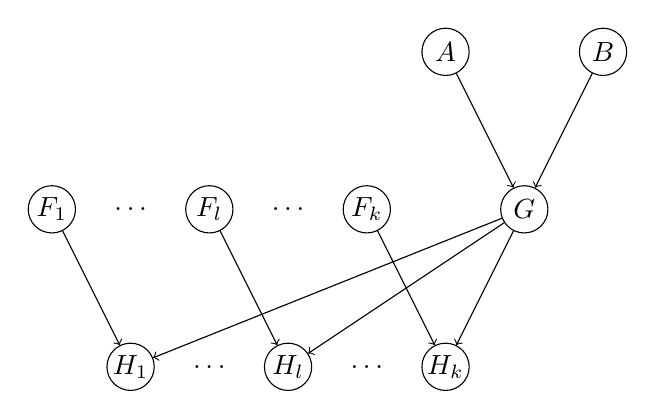
\begin{tikzpicture}
\foreach \x/\y/\n/\t in {0/4/f1/F_1, 2/4/fl/F_l, 4/4/fk/F_k, 6/4/g/G, 1/2/h1/H_1, 3/2/hl/H_l, 5/2/hk/H_k, 5/6/a/A, 7/6/b/B}
  \node[inner sep=0mm,circle,draw,minimum size=6mm] (\n) at (\x,\y) {$\t$};
\foreach \x/\y/\n/\t in {1/4/fdots1/\ldots, 3/4/fdots2/\ldots, 2/2/hdots1/\ldots, 4/2/hdots2/\ldots}
  \node[inner sep=0mm] (\n) at (\x,\y) {$\t$};
\foreach \s/\t in {f1/h1, fl/hl, fk/hk, a/g, b/g, g/h1, g/hl, g/hk}
  \draw[->] (\s) -- (\t);

\end{tikzpicture}
\end{center}

\emph{Case 1.} Suppose that there is $l$ such that $\lef(F_l) \leq \lef(G)$. If $\lef(F_l) < \lef(G)$, then $F_l$ must contain all variables $x_i, \ldots, x_j$, since otherwise either $F_l$ or $H_l$ will have smaller $\tup$ then $G$. Thus $F_l$ contains $A$. Then, we can restructure the circuit by feeding $B$ to $H_l$ instead of $G$. This does not change the value of the gate computed by $H_l$ and reduces $\out(G)$. Thus $\tup({\cal C})$ increases and we are done.

If $\lef(F_l) = \lef(G)$, then $F_l$ still cannot have gap variables among $x_i, \ldots, x_{j-1}$ as it would contradict the minimality of $G$. Thus, $F_l$ is either a range, or it is not a range, but contain all variables $x_i, \ldots, x_{j-1}$. In the latter case again $F_l$ contains $A$. In the former case $F_l$ either contains $A$, or is contain in $G$. If $F_l$ contains $A$, we can again simplify the circuit as above. If $F_l$ is contained in $G$, we have $G=H_l$, so we can remove $H_l$ from the circuit and reduce the size of the circuit.

\emph{Case 2.} Suppose that for all $l$ we have $\lef(F_l)>\lef(G)$. Consider $l$ such that $F_l$ has the minimal $\righ(F_l)$ (if there are several such $l$ pick among them the one with the minimal $\num(F_l)$). For convenience of notation let $l=k$. Now we restructure the circuit in the following way. We feed $F_k$ to $G$ instead of $A$. We feed $A$ to $H_k$ instead of $F_k$. We feed $H_k$ to all other $H_p$'s instead of $G$.

\begin{center}
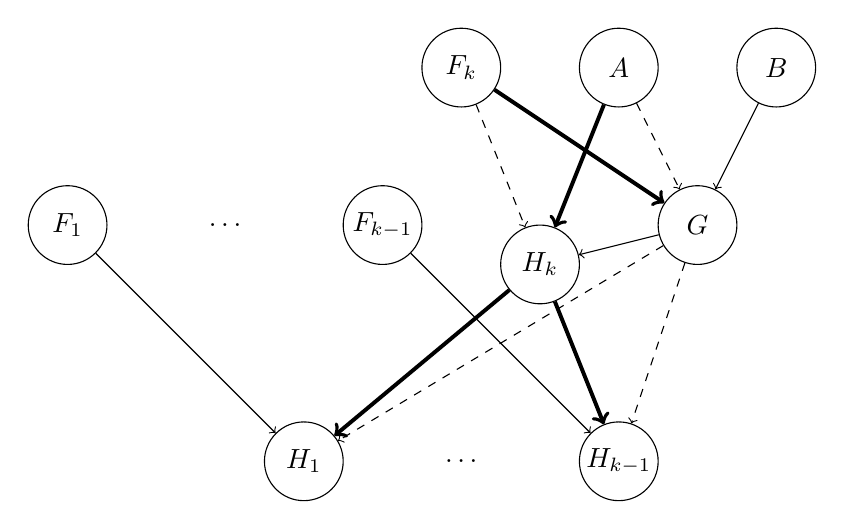
\begin{tikzpicture}
\foreach \x/\y/\n/\t in {-2/4/f1/F_1, 2/4/fk1/F_{k-1}, 3/6/fk/F_k, 6/4/g/G, 1/1/h1/H_1, 5/1/hk1/H_{k-1}, 4/3.5/hk/H_k, 5/6/a/A, 7/6/b/B}
  \node[inner sep=0mm,circle,draw,minimum size=10mm] (\n) at (\x,\y) {$\t$};
\foreach \x/\y/\n/\t in {0/4/fdots1/\ldots, 3/1/hdots1/\ldots}
  \node[inner sep=0mm] (\n) at (\x,\y) {$\t$};
\foreach \s/\t in {f1/h1, fk1/hk1, b/g, g/hk}
  \draw[->] (\s) -- (\t);
\foreach \s/\t in {fk/hk, a/g, g/h1, g/hk1}
  \draw[->,dashed] (\s) -- (\t);
\foreach \s/\t in {fk/g, a/hk, hk/h1, hk/hk1}
  \draw[->,line width=0.5mm] (\s) -- (\t);

\end{tikzpicture}
\end{center}

Observe that all these reconstructions are valid, that is, they do not create directed cycles in the circuit. To verify this we need to check that there are no cycles using new edges. Indeed, there cannot be a cycle going through one of the edges $(H_k,H_p)$ since this would mean that there was a directed path from $H_p$ to one of the vertices $F_k$, $A$ and $G$ on the original circuit. Such a path to $A$ or $G$ would mean a cycle in the original circuit. Such a path to $F_k$ violates the minimality property of $F_k$ (minimal $\righ(F_k)$). Next, there cannot be a cycle going through both edges $(F_k,G)$ and $(A,H_k)$, since substituting these edges by $(F_k,H_k)$ and $(A,G)$ we obtain one or two cycles in the original circuit. Next, there cannot be a cycle going through the edge $(A,H_k)$ only, since $H_k$ is reachable from $A$ in the original circuit and this would mean a cycle in the original circuit. Finally, there cannot be a cycle going only through the edge $(F_k,G)$ since this would mean a directed path from $G$ to $F_k$ in the original circuit and this contradicts $\lef(F_k)>\lef(G)$.

Note that our reconstruction might require reordering of the circuit gates, since we create edges between previously incomparable $H$-gates and between $F_k$ and $G$. But the reordering affect only the gates with $\num$ greater than $\num(G)$ and may only reduce $\num(F_k)$ to be smaller than $\num(G)$. But this can only increase $\tup(G)$ and since $\lef(F_k)>\lef(G)$ this can only increase $\tup({\cal C})$.

Observe, that the circuit still computes the outputs correctly. The changes are in the gates $H_1\ldots, H_k$ (and also in $G$, but $H_1,\ldots, H_k$ are all of its outputs). $H_k$ does not change. Other $H_p$'s might have changed, they now additionally include variables of $F_k$. But note that all of these variables are in between of $\lef(H_p)$ and $\righ(H_p)$, so they must be presented in the output gates connected to $H_p$ anyway (recall that at the output gates we compute ranges).

Now, observe that $\tup(G)$ has increased (by the first coordinate). There are no new gates with smaller $\lef$. Among gates with the minimal $\lef$ there are no new gates with smaller $\gap$. Among gates with minimal $(\lef,\gap)$ all gates have larger $\num$ then $G$. Thus $\tup({\cal C})$ increased and we are done.
\end{proof}